% ***************************************************************************************************
%
%	Szablon pracy magisterskiej dla Politechniki Wrocławskiej w wersji dwustronnej.
%	Autor:	Tomasz Strzałka
% Koretkta i dostosowanie do wymogów WIT 3.12.2021: dr inż. Anna Lauks-Dutka
%
% ***************************************************************************************************

% Styl dwustronny z domyślną wielkością czcionki 10pt oraz oddzieloną stroną tytułową (titlepage).
% Domyślnie rodziały rozpoczynają się na stronie prawej (openright).
\documentclass[10pt]{book}
\usepackage{times}


% ***************************************************************************************************
% Ustawienia języka
% ***************************************************************************************************

% Podstawowe ustawienia języka, według którego formatowany będzie dokument
\usepackage[polish]{babel}

% Pakiet babel dla polskiego języka powoduje konflikt z pakietem amssymb.
% Polecenie '\lll' definiują oba pakiety - porządana jest druga definicja.
\let\lll\undefined

% W przypadku wielojęzykowości ustawia główny język dokumentu
\selectlanguage{polish}

% Kodowanie dokumentu
\usepackage[utf8]{inputenc}

% Dowolny rozmiar czcionek, kodowanie znaków
\usepackage{lmodern}

% Polskie wcięcia akapitów
\usepackage{indentfirst}

% Polskie łamanie wyrazów
\usepackage[plmath]{polski}

% Przecinek w wyrażeniach matematycznych zamiast kropki
\usepackage{icomma}

% Polskie formatowanie typograficzne
\frenchspacing

% Zapewnia liczne usprawnienia wyświetlania i organizacji matematycznych formuł. 
\usepackage{amsmath}

% Wprowadza rozszerzony zestaw symboli m.in. \leadsto
\usepackage{amssymb}

% Dodatkowa, ,,kręcona'' czcionka matematyczna
\usepackage{mathrsfs}

% Dodatkowe wsparcie dla środowiska mathbb, które nie wspiera domyślnie cyfr (\mathbb{})
\usepackage{bbold}

% Fixes/improves amsmath
\usepackage{mathtools}


% ***************************************************************************************************
% Kolory  
% ***************************************************************************************************

% Umożliwia kolorowanie poszczególnych komórek tabeli
\usepackage[table]{xcolor}% http://ctan.org/pkg/

% Umożliwia łatwą zmianę koloru linii w tabeli
\usepackage{tabu}

% Umożliwia rozszerzoną kontrolę nad kolorami.
\usepackage{xcolor}

% Definicje kolorów
\definecolor{lgray}{HTML}{9F9F9F}
\definecolor{dgray}{HTML}{5F5F5F}
% lgray				-	nazwa nowo zdefiniowanego koloru
% HTML				-	model kolorów
% CCCCCC			-	wartość koloru zgodna z modelem

% ***************************************************************************************************
% Algorytmy 
% ***************************************************************************************************

% Udostępnia środowisko do konstruowania pseudokodów
\usepackage[ruled,vlined,linesnumbered,longend,algochapter]{algorithm2e}
% ruled	- poziome kreski na początku i końcu algorytmu, podpis na górze oddzielony również kreską poziomą
% vlined - pionowe kreski łączące początek polecenia z jego końcem
% linesnumbered	- numerowanie kolejnych wierszy algorytmu
% longend - długie końcówki np. ifend, forend itd.
% algochapter - numeracja z rozdziałami

% Zamiana nazwy środowiska z domyślnej "Algorithm X" na "Pseudokod X"
\newenvironment{pseudokod}[1][htb]{
	\renewcommand{\algorithmcfname}{Pseudokod}
	\begin{algorithm}[#1]%
	}{
\end{algorithm}
}

% Zmiana rozmiaru komentarzy
\newcommand\algcomment[1]{
	\footnotesize{#1}
}

% Ustawienie zadanego stylu dla komentarzy
\SetCommentSty{algcomment}

% Wyśrodkowana tylda
\usepackage{textcomp}%
\newcommand{\textapprox}{\raisebox{0.5ex}{\texttildelow}}

% Listowanie kodów źródłowych
\usepackage{listings} 
\renewcommand{\lstlistingname}{Kod źródłowy} % Polska nazwa listingu

% Definicje pecjalnych znaków, które nie są obsługiwane w środowisku listing
\lstset{literate=
	{ż}{{\.{z}}}1	{ź}{{\'{z}}}1
	{ć}{{\'{c}}}1	{ń}{{\'{n}}}1
	{ą}{{\c a}}1	{ś}{{\'{s}}}1
	{ł}{{\l}}1		{ę}{{\c{e}}}1
	{ó}{{\'{o}}}1	{á}{{\'a}}1
	{é}{{\'e}}1		{í}{{\'i}}1
	{ó}{{\'o}}1		{ú}{{\'u}}1
	{ù}{{\`u}}1		{Á}{{\'A}}1
	{É}{{\'E}}1		{Í}{{\'I}}1
	{Ó}{{\'O}}1		{Ú}{{\'U}}1
	{à}{{\`a}}1		{è}{{\'e}}1
	{ì}{{\`i}}1		{ò}{{\`o}}1
	{ò}{{\`o}}1		{À}{{\`A}}1
	{È}{{\'E}}1		{Ì}{{\`I}}1
	{Ò}{{\`O}}1		{Ò}{{\`O}}1
	{ä}{{\"a}}1		{ë}{{\"e}}1
	{ï}{{\"i}}1		{ö}{{\"o}}1
	{ü}{{\"u}}1		{Ä}{{\"A}}1
	{Ë}{{\"E}}1		{Ï}{{\"I}}1
	{Ö}{{\"O}}1		{Ü}{{\"U}}1
	{â}{{\^a}}1		{ê}{{\^e}}1
	{î}{{\^i}}1		{ô}{{\^o}}1
	{û}{{\^u}}1		{Â}{{\^A}}1
	{Ê}{{\^E}}1		{Î}{{\^I}}1
	{Ô}{{\^O}}1		{Û}{{\^U}}1
	{œ}{{\oe}}1		{Œ}{{\OE}}1
	{æ}{{\ae}}1		{Æ}{{\AE}}1
	{ß}{{\ss}}1		{ç}{{\c c}}1
	{Ç}{{\c C}}1	{ø}{{\o}}1
	{å}{{\r a}}1	{Å}{{\r A}}1
	{€}{{\EUR}}1	{£}{{\pounds}}1
}

% ***************************************************************************************************
% Marginesy 
% ***************************************************************************************************

% Ustawienia rozmiarów stron i ich marginesów
%korekta ALD - dodatkowe 0.5cm na oprawę z lewej
%\usepackage[headheight=18pt, top=25mm, bottom=25mm, left=25mm, right=25mm]{geometry}
\usepackage[headheight=18pt, top=25mm, bottom=25mm, left=30mm, right=25mm]{geometry}
% headheight		-	wysokość tytułów
% top				-	margines górny
% bottom			-	margines dolny
% left				-	margines lewy
% right				-	margines prawy

% Usunięcie górnego marginesu dla środowisk
\makeatletter
\setlength\@fptop{0\p@}	
\makeatother

% ***************************************************************************************************
% Styl 
% ***************************************************************************************************

% Definiuje środowisko 'titlingpage', które zapewnia pełną kontrolę nad układem strony tytułowej.
\usepackage{titling}


% Umożliwia modyfikowanie stylu spisu treści
\usepackage{tocloft}	

\tocloftpagestyle{tableOfContentStyle}

% Definiowanie własnych stylów nagłówków i/lub stopek
\usepackage{fancyhdr}

% Domyślny styl dla pracy 
\fancypagestyle{custom}{
	\fancyhf{}									% wyczyść stopki i nagłówki
	\fancyhead[RO]{								% Prawy, nieparzysty nagłówek
%korekta ALD: 
%\hrulefill \hspace{16pt} \large Rozdział \thechapter
		\hrulefill \hspace{16pt} \large \ifnum \thechapter>0 {Rozdział \thechapter} \else{Wstęp}\fi
		\put(-472.1, 12.1){%
			\makebox(0,0)[l]{%
                
\includegraphics[width=0.05\textwidth]{logotypy/uczelnia-logo}
			}
		}
		\put(-443,5.5){%
			\makebox(0,0)[l]{%
				\small Akademia Ekonomiczno-Humanistyczna w Warszawie
			}
		}
	}
	\fancyhead[LE]{								% Lewy, parzysty nagłówek
%korekta ALD: 
%\large Rozdział \thechapter \hspace{16pt} \hrulefill 
        \large \ifnum \thechapter>0 {Rozdział \thechapter} \else{Wstęp}\fi \hspace{16pt} \hrulefill 
		\put(-22, 12.1){%
			\makebox(0,0)[l]{%
                %korekta ALD
				%\includegraphics[width=0.05\textwidth]{pwr-logo}
                
\includegraphics[width=0.05\textwidth]{logotypy/wydzial-logo}			}
		}
		\put(-210,5.5){%
			\makebox(0,0)[l]{%
%				\small Wydział Podstawowych Problemów Techniki
%Korekta ALD
\small Wydział Technologii Informatycznych
			}
		}
	}
	\fancyfoot[LE,RO]{							% Stopki
		\thepage
	}
	\renewcommand{\headrulewidth}{0pt}			% Grubość linii w nagłówku
	\renewcommand{\footrulewidth}{0.2pt}		% Grubość linii w stopce
}


% Domyślny styl dla bibliografii
\fancypagestyle{bibliographyStyle}{
	\fancyhf{}									% wyczyść stopki i nagłówki
	\fancyhead[RO]{								% Prawy, nieparzysty nagłówek
		\hrulefill \hspace{16pt} \large Dodatek \thechapter
		\put(-472.1, 12.1){%
			\makebox(0,0)[l]{%
	
\includegraphics[width=0.05\textwidth]{logotypy/uczelnia-logo}
			}
		}
		\put(-443,5.5){%
			\makebox(0,0)[l]{%
				\small Akademia Ekonomiczno-Humanistyczna w Warszawie
			}
		}
	}
	\fancyhead[LE]{								% Lewy, parzysty nagłówek
		\large Bibliografia \hspace{16pt} \hrulefill 
		\put(-22, 12.1){%
			\makebox(0,0)[l]{%
			%korekta ALD	\includegraphics[width=0.05\textwidth]{wppt-logo}
			
\includegraphics[width=0.05\textwidth]{logotypy/wydzial-logo}
			}
		}
		\put(-210,5.5){%
			\makebox(0,0)[l]{%
			%korekta ALD
				%\small Wydział Podstawowych Problemów Techniki
				\small Wydział Technologii Informatycznych
			}
		}
	}
	\fancyfoot[LE,RO]{							% Stopki
		\thepage
	}
	\renewcommand{\headrulewidth}{0pt}			% Grubość linii w nagłówku
	\renewcommand{\footrulewidth}{0.2pt}		% Grubość linii w stopce
}

% Domyślny styl dla spisu tabel i rysunków
\fancypagestyle{listOfTablesStyle}{
	\fancyhf{}									% wyczyść stopki i nagłówki
	\fancyhead[RO]{								% Prawy, nieparzysty nagłówek
		\hrulefill \hspace{16pt} \large Spis tabel
		\put(-472.1, 12.1){%
			\makebox(0,0)[l]{%
			
\includegraphics[width=0.05\textwidth]{logotypy/uczelnia-logo}
			}
		}
		\put(-443,5.5){%
			\makebox(0,0)[l]{%
				\small Akademia Ekonomiczno-Humanistyczna w Warszawie
			}
		}
	}
	\fancyhead[LE]{								% Lewy, parzysty nagłówek
		\large Spis tabel \hspace{16pt} \hrulefill 
		\put(-22, 12.1){%
			\makebox(0,0)[l]{%

\includegraphics[width=0.05\textwidth]{logotypy/wydzial-logo}
			}
		}
		\put(-210,5.5){%
			\makebox(0,0)[l]{%
				\small Wydział Technologii Informatycznych
			}
		}
	}
	\fancyfoot[LE,RO]{							% Stopki
		\thepage
	}
	\renewcommand{\headrulewidth}{0pt}			% Grubość linii w nagłówku
	\renewcommand{\footrulewidth}{0.2pt}		% Grubość linii w stopce
}

\fancypagestyle{listOfPlotsStyle}{
	\fancyhf{}									% wyczyść stopki i nagłówki
	\fancyhead[RO]{								% Prawy, nieparzysty nagłówek
		\hrulefill \hspace{16pt} \large Spis rysunków
		\put(-472.1, 12.1){%
			\makebox(0,0)[l]{%
			
\includegraphics[width=0.05\textwidth]{logotypy/uczelnia-logo}
			}
		}
		\put(-443,5.5){%
			\makebox(0,0)[l]{%
				\small Akademia Ekonomiczno-Humanistyczna w Warszawie
			}
		}
	}
	\fancyhead[LE]{								% Lewy, parzysty nagłówek
		\large Spis rysunków \hspace{16pt} \hrulefill 
		\put(-22, 12.1){%
			\makebox(0,0)[l]{%

\includegraphics[width=0.05\textwidth]{logotypy/wydzial-logo}
			}
		}
		\put(-210,5.5){%
			\makebox(0,0)[l]{%
				\small Wydział Technologii Informatycznych
			}
		}
	}
	\fancyfoot[LE,RO]{							% Stopki
		\thepage
	}
	\renewcommand{\headrulewidth}{0pt}			% Grubość linii w nagłówku
	\renewcommand{\footrulewidth}{0.2pt}		% Grubość linii w stopce
}

% Domyślny styl dla dodatków
\fancypagestyle{appendixStyle}{
	\fancyhf{}									% wyczyść stopki i nagłówki
	\fancyhead[RO]{								% Prawy, nieparzysty nagłówek
		\hrulefill \hspace{16pt} \large Załącznik \thechapter
		\put(-472.1, 12.1){%
			\makebox(0,0)[l]{%

\includegraphics[width=0.05\textwidth]{logotypy/uczelnia-logo}
			}
		}
		\put(-443,5.5){%
			\makebox(0,0)[l]{%
				\small Akademia Ekonomiczno-Humanistyczna w Warszawie
			}
		}
	}
	\fancyhead[LE]{								% Lewy, parzysty nagłówek
		\large Załącznik \thechapter \hspace{16pt} \hrulefill 
		\put(-22, 12.1){%
			\makebox(0,0)[l]{%
%korekta ALD:				\includegraphics[width=0.05\textwidth]{wppt-logo}

\includegraphics[width=0.05\textwidth]{logotypy/wydzial-logo}
			}
		}
		\put(-210,5.5){%
			\makebox(0,0)[l]{%
			%korekta ALD
				%\small Wydział Podstawowych Problemów Techniki
				\small Wydział Technologii Informatycznych
			}
		}
	}
	\fancyfoot[LE,RO]{							% Stopki
		\thepage
	}
	\renewcommand{\headrulewidth}{0pt}			% Grubość linii w nagłówku
	\renewcommand{\footrulewidth}{0.2pt}		% Grubość linii w stopce
}

% Osobny styl dla stron zaczynających rozdział/spis treści itd. (domyślnie formatowane jako "plain")
\fancypagestyle{chapterBeginStyle}{
	\fancyhf{}%
	\fancyfoot[LE,RO]{
		\thepage
	}
	\renewcommand{\headrulewidth}{0pt}
	\renewcommand{\footrulewidth}{0.2pt}
}

% Styl dla pozostałych stron spisu treści
\fancypagestyle{tableOfContentStyle}{
	\fancyhf{}%
	\fancyfoot[LE,RO]{
		\thepage
	}
	\renewcommand{\headrulewidth}{0pt}
	\renewcommand{\footrulewidth}{0.2pt}
}
% Formatowanie tytułów rozdziałów i/lub sekcji
\usepackage{titlesec}

% Formatowanie tytułów rozdziałów
\titleformat{\chapter}[hang]					% kształt
{
	\vspace{-10ex}
	%\Huge
	\large
	\bfseries
}												% formatowanie tekstu modyfikowanego elementu
{}												% etykieta występująca przed tekstem modyfikowanego elementu, niewidoczna w spisie treści
{
	10pt
}												% odstęp formatowanego tytułu od lewego marginesu/etykiety
{
    \large
	\bfseries
}												% formatowanie elementów przed modyfikowanym tytułem
[
\vspace{2ex}
%\rule{\textwidth}{0.4pt}
%\vspace{-4ex}
]												% dodatkowe formatowanie stosowane poniżej modyfikowanego tytułu


% Formatowanie tytułów sekcji
\titleformat{\section}[hang]					% kształt
{
	\vspace{2ex}
%	\titlerule\vspace{1ex}
	\large\bfseries
}												% formatowanie tekstu modyfikowanego elementu
{
	\thesection									% etykieta występująca przed tekstem modyfikowanego elementu, niewidoczna w spisie treści
}
{
	0pt
}												% odstęp formatowanego tytułu od lewego marginesu/etykiety
{
	\large
	\bfseries
}												% formatowanie elementów przed modyfikowanym tytułem


%ALD- ustawienia wielkości fontów dla rozdziałów i sekcji
\usepackage{sectsty}
%\chapterfont{\fontsize{14}{17.6}\selectfont}
\sectionfont{\fontsize{13}{16.8}\selectfont}
\subsectionfont{\fontsize{12}{15.6}\selectfont}

% ***************************************************************************************************
% Linki
% ***************************************************************************************************

% Umożliwia wstawianie hiperłączy do dokumentu
\usepackage{hyperref}							% Aktywuje linki

\hypersetup{
	colorlinks	=	true,					% Koloruje tekst zamiast tworzyć ramki.
	linkcolor		=	blue,					% Kolory: referencji,
        citecolor		=	blue,					% cytowań,
	urlcolor		=	blue					% hiperlinków.
}

% Do stworzenia hiperłączy zostanie użyta ta sama (same) czcionka co dla reszty dokumentu
\urlstyle{same}




% ***************************************************************************************************
% Linki
% ***************************************************************************************************

% Umożliwia zdefiniowanie własnego stylu wyliczeniowego
\usepackage{enumitem}

% Nowa lista numerowana z trzema poziomami
\newlist{myitemize}{itemize}{3}

% Definicja wyglądu znacznika pierwszego poziomu
\setlist[myitemize,1]{
	label		=	\textbullet,
	leftmargin	=	4mm}

% Definicja wyglądu znacznika drugiego poziomu
\setlist[myitemize,2]{
	label		=	$\diamond$,
	leftmargin	=	8mm}

% Definicja wyglądu znacznika trzeciego poziomu
\setlist[myitemize,3]{
	label		=	$\diamond$,
	leftmargin	=	12mm
}

% ***************************************************************************************************
% Inne pakiety
% ***************************************************************************************************

% Dołączanie rysunków
\usepackage{graphicx}

% Figury i przypisy
\usepackage{caption}
\usepackage{subcaption}

% Umożliwia tworzenie przypisów wewnątrz środowisk
\usepackage{footnote}

% Umożliwia tworzenie struktur katalogów
\usepackage{dirtree}

% Rozciąganie komórek tabeli na wiele wierszy
\usepackage{multirow}

% Precyzyjne obliczenia szerokości/wysokości dowolnego fragmentu wygenerowanego przez LaTeX
\usepackage{calc}

% ***************************************************************************************************
% Matematyczne skróty
% ***************************************************************************************************

% Skrócony symbol liczb rzeczywistych
\newcommand{\RR}{\mathbb{R}}

% Skrócony symbol liczb naturalnych
\newcommand{\NN}{\mathbb{N}}

% Skrócony symbol liczb wymiernych
\newcommand{\QQ}{\mathbb{Q}}

% Skrócony symbol liczb całkowitych
\newcommand{\ZZ}{\mathbb{Z}}

% Skrócony symbol logicznej implikacji
\newcommand{\IMP}{\rightarrow}

% Skrócony symbol  logicznej równoważności
\newcommand{\IFF}{\leftrightarrow}

% ***************************************************************************************************
% Środowiska
% ***************************************************************************************************

% Środowisko do twierdzeń
\newtheorem{theorem}{Twierdzenie}[chapter]

% Środowisko do lematów
\newtheorem{lemma}{Lemat}[chapter]

% Środowisko do przykładów
\newtheorem{example}{Przykład}[chapter]

% Środowisko do wniosków
\newtheorem{corollary}{Wniosek}[chapter]

% Środowisko do definicji
\newtheorem{definition}{Definicja}[chapter]

% Środowisko do dowodów
\newenvironment{proof}{
	\par\noindent \textbf{Dowód.}
}{
\begin{flushright}
	\vspace*{-6mm}\mbox{$\blacklozenge$}
\end{flushright}
}

%ALD - nowe środowisko do streszczenia i abstractu
\newenvironment{streszczenie}{
	\par\noindent {\large \textbf{Streszczenie}\\[14pt]\indent}
}{}
\newenvironment{abstract}{
	\par\noindent {\large \textbf{Abstract}\\[14pt]\indent}
}{}

% Środowisko do uwag
\newenvironment{remark}{
	\bigskip \par\noindent \small \textbf{Uwaga.}
}{
\begin{small}
	\vspace*{4mm}
\end{small}
}

% ***************************************************************************************************
% Słownik
% ***************************************************************************************************

% Prawidłowe dzielenie wyrazów
\hyphenation{wszy-stkich ko-lu-mnę każ-da od-leg-łość
	dzie-dzi-ny dzie-dzi-na rów-nych rów-ny
	pole-ga zmie-nna pa-ra-met-rów wzo-rem po-cho-dzi
	o-trzy-ma wte-dy wa-run-ko-wych lo-gicz-nie
	skreś-la-na skreś-la-ną cał-ko-wi-tych wzo-rów po-rzą-dek po-rząd-kiem
	przy-kład pod-zbio-rów po-mię-dzy re-pre-zen-to-wa-ne
	rów-no-waż-ne bi-blio-te-kach wy-pro-wa-dza ma-te-ria-łów
	prze-ka-za-nym skoń-czo-nym moż-esz na-tu-ral-na cią-gu tab-li-cy
	prze-ka-za-nej od-po-wied-nio}

% ***************************************************************************************************
% Dokument
% ***************************************************************************************************

\frontmatter

\begin{document}

    \pagestyle{empty}
	\begin{titlingpage}
		\vspace*{\fill}
		\begin{center}
			\begin{picture}(430,500)
				\put(0,590){\makebox(0,0)[l]{\huge \textbf{Akademia Ekonomiczno-Humanistyczna}}}
				\put(40,565){\makebox(0,0)[l]{\Large \textbf{Wydział Technologii Informatycznych}}}
                \put(0,550){\line(1,0){430}}
                \put(0,510){\makebox(0,0)[l]{\large Kierunek: \textbf{Informatyka}}}
                %\textbf{3 literowy kod kierunku}}}
                % \put(0,490){\makebox(0,0)[l]{\large Specjalność: \textbf{-}}}                
                %\textbf{3 literowy kod specjalności}}}                
				\put(0,370){\begin{minipage}{0.9\textwidth}
				\centering
				\Huge \textsc{Praca Dyplomowa\\ Magisterska}
                \end{minipage}
				}
% Tytuł pracy
				\put(0,230){\begin{minipage}{0.9\textwidth}
				\centering
				\LARGE \textbf{Efektywność Wielkich Modeli Językowych w rozwiązywaniu problemów logicznych}
                \end{minipage}
				}
% Autor pracy
				\put(0,170){\begin{minipage}{0.9\textwidth}
				\centering
				\Large {
				Krzysztof Małczak
				}
				\end{minipage}
				}
% dane promotora
				\put(0,90){\begin{minipage}{0.9\textwidth}
				\centering
				\large{
				Opiekun pracy\\
				\textbf{dr inż. Krzysztof Rychlicki-Kicior}
				}
				\end{minipage}
				}
				\put(0,-30){
				\begin{minipage}{0.9\textwidth}
				\normalsize{
				Słowa kluczowe: LLM, Generative AI, LLM Evaluation 
				}
				\end{minipage}
				}
                \put(0,-80){\line(1,0){430}}
				\put(155,-100){\makebox(0,0)[bl]{\large \textsc{Warszawa 2025}}}
			\end{picture}
		\end{center}	
		\vspace*{\fill}
	\end{titlingpage}
	
    \cleardoublepage
	\begin{streszczenie}
Tutaj tekst streszczenia po polsku. 
\end{streszczenie}

	\vspace*{1cm}	
    \begin{abstract}
Tutaj treść streszczenia po angielsku.
\end{abstract}


    \cleardoublepage
	\pagenumbering{Roman}
	\pagestyle{tableOfContentStyle}
	\tableofcontents

	% spis rysunków (opcjonalnie)    
	\clearpage
	\pagestyle{listOfPlotsStyle}
        \listoffigures
        \addcontentsline{toc}{chapter}{Spis rysunków}
        
        % spis tabel (opcjonalnie)
        \clearpage
        \renewcommand{\listtablename}{Spis tabel}    
        \pagestyle{listOfTablesStyle}
	\listoftables
	\addcontentsline{toc}{chapter}{Spis tabel}




    \cleardoublepage
    
		
	% ***************************************************************************************************
	% Wstęp
	% ***************************************************************************************************
	
	\pagestyle{custom}
	\mainmatter
	
	% ***************************************************************************************************
	% Rodziały
	% ***************************************************************************************************

	%Korekta ALD - nienumerowany wstęp
\chapter*{Wstęp}
\addcontentsline{toc}{chapter}{Wstęp}

\thispagestyle{chapterBeginStyle}

Praca dyplomowa inżynierska jest dokumentem opisującym zrealizowany system techniczny. Praca powinna być napisana poprawnym językiem odzwierciedlającym aspekty techniczne (informatyczne) omawianego zagadnienia. Praca powinna być napisana w trybie bezosobowym (w szczególności należy unikać trybu pierwszej osoby liczby pojedynczej i mnogiej). Zdania opisujące konstrukcję systemu informatycznego powinny być tworzone w stronie biernej. W poniższym dokumencie przykłady sformułowań oznaczono kolorem niebieskim. W opisie elementów systemu, komponentów, elementów kodów źródłowych, nazw plików, wejść i wyjść konsoli należy stosować czcionkę stałej szerokości, np: {\color{lgray}zmienna \verb|wynik| przyjmuje wartość zwracaną przez funkcję \verb|dodaj(a,b)|, dla argumentów \verb|a| oraz \verb|b| przekazywanych \ldots}.

Układ poniższego dokumentu przedstawia wymaganą strukturę pracy, z rozdziałami zawierającymi analizę zagadnienia, opis projektu systemu oraz implementację (dobór podrozdziałów jest przykładowy i należy go dostosować do własnej tematyki pracy). 
  
Wstęp pracy (nie numerowany) powinien składać się z czterech części (które nie są wydzielane jako osobne podrozdziały): zakresu pracy, celu, analizy i porównania istniejących rozwiązań oraz przeglądu literatury, oraz opisu zawartości pracy.

Każdy rozdział powinien rozpoczynać się od akapitu wprowadzającego, w którym zostaje w skrócie omówiona zawartość tego rozdziału.

{\color{dgray}
Praca swoim zakresem obejmuje wielowarstwowe rozproszone systemy informatyczne typu ,,B2B'' wspierające wymianę danych pomiędzy przedsiębiorstwami. Systemy tego typu, konstruowane dla dużych korporacji, charakteryzują się złożoną strukturą poziomą i pionową, w której dokumenty \ldots

Celem pracy jest zaprojektowanie i oprogramowanie aplikacji o następujących założeniach funkcjonalnych:
\begin{itemize}
    \item wspieranie zarządzania obiegiem dokumentów wewnątrz korporacji z uwzględnieniem \ldots,
	\item wspieranie zarządzania zasobami ludzkimi z uwzględnieniem modułów kadrowych oraz \ldots,
	\item gotowość do uzyskania certyfikatu ISO \ldots,
	\item \ldots.
\end{itemize}

Istnieje szereg aplikacji o zbliżonej funkcjonalności: \ldots, przy czym \ldots.

Praca składa się z czterech rozdziałów.
W rozdziale pierwszym omówiono strukturę przedsiębiorstwa \ldots, scharakteryzowano grupy użytkowników oraz przedstawiono procedury związane z obiegiem dokumentów. Szczegółowo opisano mechanizmy \ldots. Przedstawiono uwarunkowania prawne udostępniania informacji \ldots, w ramach \ldots.

W rozdziale drugim przedstawiono szczegółowy projekt systemy w notacji UML. Wykorzystano diagramy \ldots.
Opisano w pseudokodzie i omówiono algorytmy generowania \ldots.

W rozdziale trzecim opisano technologie implementacji projektu: wybrany język programowania, biblioteki, system zarządzania bazą danych, itp.  Przedstawiono dokumentację techniczną kodów źródłowych interfejsów poszczególnych modułów systemu. Przedstawiono sygnatury metod publicznych oraz \ldots.

W rozdziale czwartym przedstawiono sposób instalacji i wdrożenia systemu w środowisku docelowym.

Końcowy rozdział stanowi podsumowanie uzyskanych wyników.
}


	\cleardoublepage

	\chapter{Analiza problemu}
\thispagestyle{chapterBeginStyle}
\label{rozdzial1}

W tym rozdziale należy przedstawić analizę zagadnienia, które podlega informatyzacji. Należy zidentyfikować i opisać obiekty składowe rozważanego wycinka rzeczywistości i ich wzajemne relacje (np.\ użytkowników systemu i ich role). Należy szczegółowo omówić procesy jakie zachodzą w systemie i które będą informatyzowane, takie jak np.\ przepływ dokumentów.
Należy sprecyzować i wypunktować założenia funkcjonalne i poza funkcjonalne dla projektowanego systemu.
Jeśli istnieją aplikacje realizujące dowolny podzbiór zadanych funkcjonalności realizowanego systemu należy przeprowadzić ich analizę porównawczą, wskazując na różnice bądź innowacyjne elementy, które projektowany w pracy system informatyczny będzie zawierał.
Należy odnieść się do uwarunkowań prawnych związanych z procesami przetwarzania danych w projektowanym systemie.
Jeśli zachodzi konieczność, należy wprowadzić i omówić model matematyczny elementów systemu na odpowiednim poziomie abstrakcji.

{\color{dgray}
W niniejszym rozdziale omówiono koncepcję architektury programowej systemu \ldots. W
szczególny sposób \ldots. Omówiono założenia funkcjonalne i niefunkcjonalne podsystemów \ldots. Przedstawiono
mechanizmy \ldots. Sklasyfikowano systemy ze względu na \ldots. Omówiono istniejące rozwiązania informatyczne o podobnej funkcjonalności \ldots (zobacz \cite{JCINodesChord}).
}



	\cleardoublepage

	\chapter{Projekt systemu}
\thispagestyle{chapterBeginStyle}

{\color{dgray}
W tym rozdziale przedstawiono szczegółowy projekt systemy w notacji UML uwzględniający wymagania funkcjonalne opisane w rozdziale~\ref{rozdzial1}. Do opisu relacji pomiędzy składowymi systemu wykorzystano diagramy \ldots.
Przedstawiono w pseudokodzie i omówiono algorytmy generowania \ldots.
}


\section{Grupy użytkowników i założenia}

{\color{dgray}
Architektura systemu \ldots jest wielowarstwowa i rozproszona, przy czym \ldots. Podsystem  \ldots jest systemem zbiorczym dla danych \ldots wysyłanych do serwera \ldots. 

Taka architektura jest zgodna z wzorcem projektowym MVC\footnote{Należy odnieść się do wykorzystywanych wzorców projektowych} (ang.  Model-View-Controller). Przetwarzanie danych odbywa się \ldots.
} 

\section{Przypadki użycia i scenariusze}

W tej sekcji należy przedstawić przypadki użycia oraz odpowiadające im scenariusze dla poszczególnych grup użytkowników \ldots.

\section{Diagramy klas}

W tej sekcji należy przedstawić diagramy klas dla odpowiednich elementów systemu zidentyfikowane na podstawie wcześniejszych rozważań 

\section{Diagramy aktywności}

W tej sekcji należy przedstawić diagramy aktywności dla elementów systemu i odpowiednich procesów wynikające z wcześniejszej analizy.  

{\color{dgray}
W niniejszym rozdziale przedstawiono diagramy aktywności \ldots. Diagram na rysunku~\ref{czynnosci_GD} przedstawia \ldots.
} 

\begin{figure}[h!]
\begin{center}
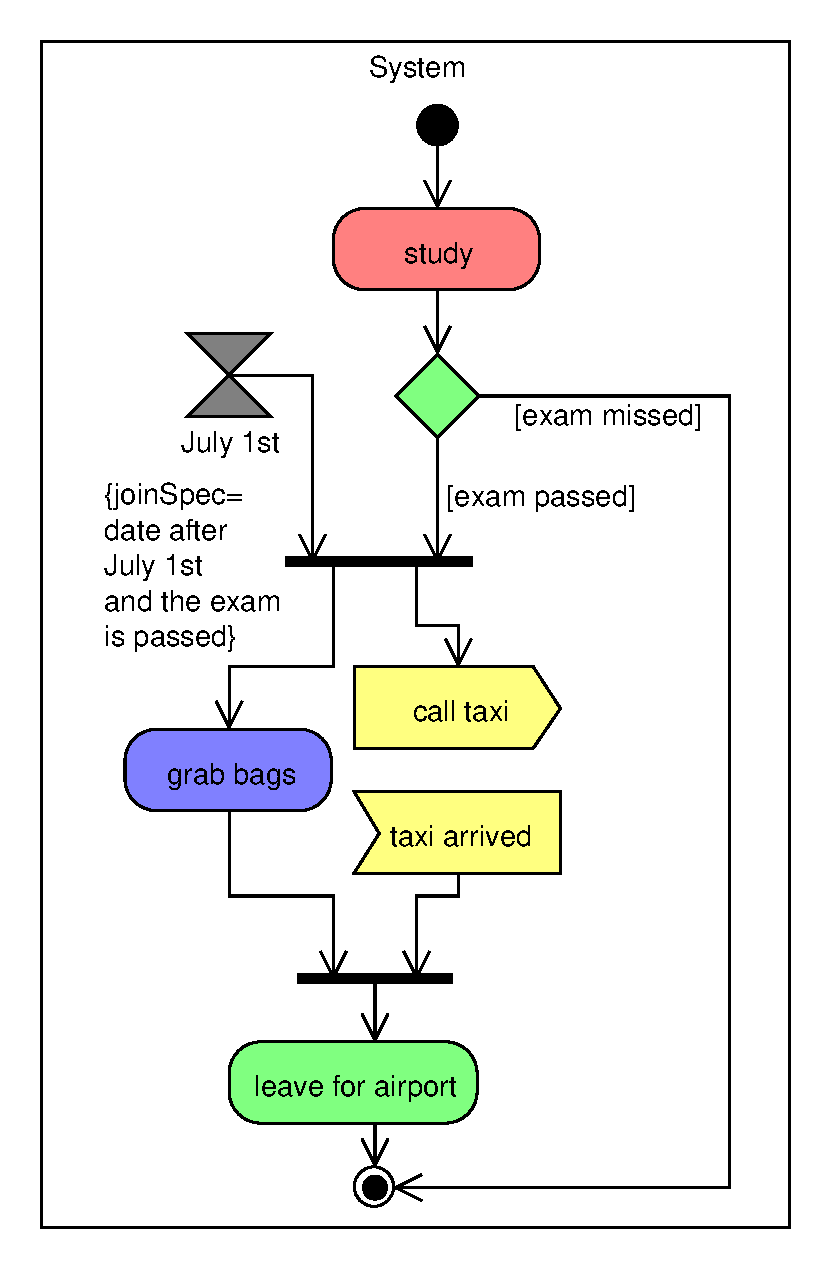
\includegraphics[width=0.5\textwidth]{./rysunki/aktyw.pdf}
\end{center}
\caption{{\color{dgray}Diagram aktywności związany z procesem rejestracji dokumentu.}} \label{czynnosci_GD}
\end{figure}  

\section{Diagramy sekwencji}

W tej sekcji należy przedstawić diagramy sekwencji dla obiektów systemu zidentyfikowanych na podstawie wcześniejszych rozważań. Należy wykorzystać nazewnictwo wprowadzone w poprzednich rozdziałach, w szczególności odpowiadające definicjom wprowadzonych klas.

\section{Diagramy stanów}

W tej sekcji należy przedstawić diagramy stanów w których może znaleźć się system. Diagramy te są szczególnie istotne przy projektowaniu systemów czasu rzeczywistego. 

\section{Projekt bazy danych}

W tej sekcji należy przedstawić projekt bazy danych. Należy omówić wycinek rzeczywistości i odpowiadające mu zidentyfikowane elementy systemu, których wartości będą podlegać utrwalaniu. Należy przedyskutować wybór typów danych dla atrybutów poszczególnych obiektów. Należy uzasadnić wybór platformy DBMS. Dla relacyjnych baz danych należy przedyskutować jej normalizację.

\section{Opis protokołów}

W tej sekcji należy omówić protokoły wykorzystywane przez komponenty systemu. Omówić formaty komunikatów i zilustrować je przykładami. 

\section{Opis algorytmów}

W tej sekcji należy wymienić i przedyskutować algorytmy wykorzystywane w systemie. Algorytmy należy przedstawić w pseudokodzie (wykorzystać pakiet \texttt{algorithm2e}). Omówienia poszczególnych kroków algorytmów powinny zawierać odwołania do odpowiednich linii pseudokodu. Dla zaproponowanych autorskich algorytmów należy przeprowadzić analizę ich złożoności czasowej i pamięciowej. 

{\color{dgray}
Algorytm bąblowania jest przedstawiony w Pseudokodzie~\ref{alg:mine}.
}

{\small
\begin{pseudokod}[H]
%\SetAlTitleFnt{small}
\SetArgSty{normalfont}
\SetKwFunction{Process}{Process}
\SetKwFunction{Calculate}{Calculate}
\KwIn{Zbiór bąbli $B$}
\KwOut{Wyporność $W$}
\ForEach{$b \in B$}{
\Process{$b$}\;
\For{$i \leftarrow 1$ \KwTo $|B|$}{
\If{\Calculate{EW($i$,$b$)} $\le$ 0}{
$b \leftarrow 2*b$\;
}
}
}
\While{$B \neq \emptyset$}{
\For{$j \leftarrow 1$ \KwTo $|B|$}{
\If{\Calculate{FT($j$,$\hat{b}$)} $\le 0$}{
$w \leftarrow 2*\hat{b}$\;
$W \leftarrow W \cup \{w\}$\;
$B \leftarrow B \setminus \{b\}$\;
}
}
}
\caption{Wyporność przez bąblowanie}\label{alg:mine}
\end{pseudokod}
}


	\cleardoublepage
	
	\chapter{Implementacja systemu}
\thispagestyle{chapterBeginStyle}

\section{Opis technologii}

Należy tutaj zamieścić krótki opis (z referencjami) do technologii użytych przy implementacji systemu.

{\color{dgray}
Do implementacji systemu użyto języka JAVA w wersji \ldots, szczegółowy opis można znaleźć w \cite{Java}. Interfejs zaprojektowano w oparciu o HTML5 i CSS3 \cite{HTML-CSS}.
}

\section{Omówienie kodów źródłowych}

{\color{dgray}
Kod źródłowy~\ref{ws} przedstawia opisy poszczególnych metod interfejsu: \texttt{WSPodmiotRejestracjaIF}. Kompletne
kody źródłowe znajdują się na płycie CD dołączonej do niniejszej pracy w katalogu \texttt{Kody} (patrz Dodatek~\ref{plytaCD}).
}

\begin{small}
\begin{lstlisting}[language=Java, frame=lines, numberstyle=\tiny, stepnumber=5, caption=Interfejs usługi Web Service: \texttt{WSPodmiotRejestracjaIF}\label{ws}., firstnumber=1]
package erejestracja.podmiot;
import java.rmi.RemoteException;
// Interfejs web serwisu dotyczącego obsługi podmiotów i rejestracji.
public interface WSPodmiotRejestracjaIF extends java.rmi.Remote{
// Pokazuje informacje o danym podmiocie.
// parametr: nrPeselRegon - numer PESEL podmiotu lub numer REGON firmy.
// return: Podmiot - obiekt transportowy: informacje o danym podmiocie.
public Podmiot pokazPodmiot(long nrPeselRegon) throws RemoteException;
// Dodaje nowy podmiot.
// parametr: nowyPodmiot - obiekt transportowy: informacje o nowym podmiocie.
// return: true - jeśli podmiot dodano, false - jeśli nie dodano.
public boolean dodajPodmiot(Podmiot nowyPodmiot) throws RemoteException;
// Usuwa dany podmiot.
// parametr: nrPeselRegon - numer PESEL osoby fizycznej lub numer REGON firmy.
// return: true - jeśli podmiot usunięto, false - jeśli nie usunięto.
public boolean usunPodmiot(long nrPeselRegon) throws RemoteException;
// Modyfikuje dany podmiot.
// parametr: podmiot - obiekt transportowy: informacje o modyfikowanym podmiocie.
// return: true - jeśli podmiot zmodyfikowano, false - jeśli nie zmodyfikowano.
public boolean modyfikujPodmiot(Podmiot podmiot) throws RemoteException;
// Pokazuje zarejestrowane podmioty na dany dowód rejestracyjny.
// parametr: nrDowoduRejestracyjnego - numer dowodu rejestracyjnego.
// return: PodmiotRejestracja[] - tablica obiektów transportowych: informacje o
// wszystkich zarejestrowanych podmiotach.
public PodmiotRejestracja[] pokazZarejestrowanePodmioty(
String nrDowoduRejestracyjnego) throws RemoteException;
// Nowa rejestracja podmiotu na dany dowód rejestracyjny.
// parametr: nrDowoduRejestracyjnego - numer dowodu rejestracyjnego.
// parametr: nrPeselRegon - numer PESEL podmiotu lub numer REGON firmy.
// parametr: czyWlasciciel - czy dany podmiot jest właścicielem pojazdu.
// return: true - jeśli zarejestrowano podmiot, false - jeśli nie zarejestrowano.
public boolean zarejestrujNowyPodmiot(String nrDowoduRejestracyjnego,
long nrPeselRegon, boolean czyWlasciciel) throws RemoteException;
// Usuwa wiązanie pomiędzy danym podmiotem, a dowodem rejestracyjnym.
// parametr: nrDowoduRejestracyjnego - numer dowodu rejestracyjnego.
// parametr: nrPeselRegon - numer PESEL podmiotu lub numer REGON firmy.
// return: true - jeśli podmiot wyrejestrowano, false - jeśli nie wyrejestrowano.
public boolean wyrejestrujPodmiot(String nrDowoduRejestracyjnego,
long nrPeselRegon) throws RemoteException;
\end{lstlisting} 
\end{small}

{\color{dgray}
Kod źródłowy~\ref{req} przedstawia procedurę przetwarzającą żądanie. Hasz utrwalany \verb|%granulacja| wykorzystywany jest do komunikacji międzyprocesowej.
}

\begin{small}
\begin{lstlisting}[language=perl, frame=lines, caption=Przetwarzanie żądania - procedura \texttt{process\_req()}\label{req}., firstnumber=86]
sub process_req(){	
  my($r) = @_;
  $wyn = "";
  if ($r=~/get/i) {
	@reqest = split(" ",$r);
	$zad = $reqest[0];
	$ts1 = $reqest[1];
	$ts2 = $reqest[2];
	@date1 = split(/\D/,$ts1);
	@date2 = split(/\D/,$ts2);
	print "odebralem: $r"; 
	$wyn = $wyn."zadanie: $zad\n";
	$wyn = $wyn."czas_od: "."$date1[0]"."-"."$date1[1]"."-"."$date1[2]"."_"."$date1[3]".":"."$date1[4]".":"."$date1[5]"."\n";
	$wyn = $wyn."czas_do: "."$date2[0]"."-"."$date2[1]"."-"."$date2[2]"."_"."$date2[3]".":"."$date2[4]".":"."$date2[5]"."\n";		
	$wyn = $wyn.&sym_sens($ts1,$ts2);
	return $wyn;
  }
  if ($r=~/set gt/i) {
	@reqest = split(" ",$r);
	$zad = $reqest[0];
	$ts1 = $reqest[1];
	$ts2 = $reqest[2];
	$gt = $reqest[2];
	dbmopen(%granulacja,"granulacja_baza",0644);
	$granulacja{"gt"}=$gt;
	dbmclose(%granulacja);
	$wyn = "\'GT\' zmienione na: $gt";
  }		
}	
\end{lstlisting} 
\end{small}

	\cleardoublepage
	
	\chapter{Instalacja i wdrożenie}
\thispagestyle{chapterBeginStyle}

W tym rozdziale należy omówić zawartość pakietu instalacyjnego oraz założenia co do środowiska, w którym realizowany system będzie instalowany. Należy przedstawić procedurę instalacji i wdrożenia systemu. Czynności instalacyjne powinny być szczegółowo rozpisane na kroki. Procedura wdrożenia powinna obejmować konfigurację platformy sprzętowej, OS (np. konfiguracje niezbędnych sterowników) oraz konfigurację wdrażanego systemu, m.in.\ tworzenia niezbędnych kont użytkowników. Procedura instalacji powinna prowadzić od stanu, w którym nie są zainstalowane żadne składniki systemu, do stanu w którym system jest gotowy do pracy i oczekuje na akcje typowego użytkownika.


	\cleardoublepage
	
	\chapter*{Podsumowanie}
\addcontentsline{toc}{chapter}{Podsumowanie}
\thispagestyle{chapterBeginStyle}

W podsumowaniu należy określić stan zakończonych prac projektowych i implementacyjnych. Zaznaczyć, które z zakładanych funkcjonalności systemu udało się zrealizować. Omówić aspekty pielęgnacji systemu w środowisku wdrożeniowym. Wskazać dalsze możliwe kierunki rozwoju systemu, np.\ dodawanie nowych komponentów realizujących nowe funkcje.

W podsumowaniu należy podkreślić nowatorskie rozwiązania zastosowane w projekcie i implementacji (niebanalne algorytmy, nowe technologie, itp.).


	\cleardoublepage
	
	
	%%%%%%%%%%%%%%%%%%%%%%%%%%%%%%%%%%%%%%%%%%%%%%%%%%%%%%%%%%%%%%%%%%%%%%%%%%%%%%
	%%%%%%%%%%%%%%%%%%%%%%%%%%%%%%% BIBLIOGRAFIA %%%%%%%%%%%%%%%%%%%%%%%%%%%%%%%%%
	%%%%%%%%%%%%%%%%%%%%%%%%%%%%%%%%%%%%%%%%%%%%%%%%%%%%%%%%%%%%%%%%%%%%%%%%%%%%%%

	\pagestyle{bibliographyStyle}
	\bibliographystyle{plabbrv}
	\bibliography{literatura}
	\thispagestyle{chapterBeginStyle}
        \addcontentsline{toc}{chapter}{Bibliografia}
	\cleardoublepage
	
	%%%%%%%%%%%%%%%%%%%%%%%%%%%%%%%%%%%%%%%%%%%%%%%%%%%%%%%%%%%%%%%%%%%%%%%%%%%%%%
	%%%%%%%%%%%%%%%%%%%%%%%%%%%%%%%%% DODATKI %%%%%%%%%%%%%%%%%%%%%%%%%%%%%%%%%%%%
	%%%%%%%%%%%%%%%%%%%%%%%%%%%%%%%%%%%%%%%%%%%%%%%%%%%%%%%%%%%%%%%%%%%%%%%%%%%%%%
	
	\appendix
	\pagestyle{appendixStyle}
       \renewcommand{\appendixname}{Załącznik}
	
	\chapter{Zawartość płyty CD}
\thispagestyle{chapterBeginStyle}
\label{plytaCD}

W tym rozdziale należy krótko omówić zawartość dołączonej płyty CD.


	
	\cleardoublepage

\end{document}

